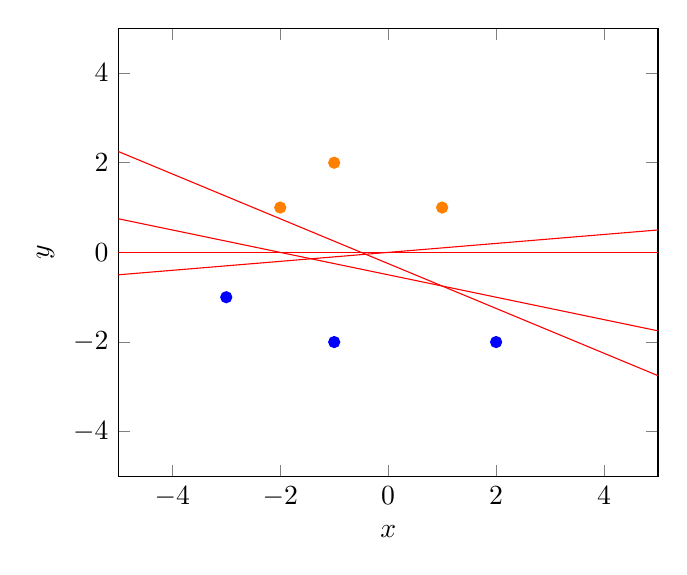
\begin{tikzpicture}

  \begin{axis}[xlabel = $x$, ylabel = $y$, xmin = -5.0, xmax = 5.0, ymin = -5.0, ymax = 5.0]
    
    \addplot[mark = *, , draw = none, color = orange] coordinates {(1,1)}; 
    \addplot[mark = *, , draw = none, color = orange] coordinates {(-1,2)}; 
    \addplot[mark = *, , draw = none, color = orange] coordinates {(-2,1)}; 

    \addplot[mark = *, , draw = none, color = blue] coordinates {(-1,-2)}; 
    \addplot[mark = *, , draw = none, color = blue] coordinates {(2,-2)}; 
    \addplot[mark = *, , draw = none, color = blue] coordinates {(-3,-1)}; 

    \addplot[color = red] {0};
    \addplot[color = red] {-0.25*x - 0.50};
    \addplot[color = red] {-0.50*x - 0.25};
    \addplot[color = red] {0.1*x};
    
    %\addplot[mark = *, , draw = none, color = red] coordinates {(-1,-1)};

  \end{axis}

\end{tikzpicture}